\lecture{2}{4. Februar 2025}{Energi og proces}

\section{Energi}

\subsection{Mikroskopiske energier for et stof}
Et stofs mikroskopiske energier er en løs betegnelse, der dækker over, ja, de mikroskopiske og dermed ``usynlige'' energier i et stof. Disse er bl.a:
\begin{itemize}
  \item \textbf{Sensibel energi:} Også kendt som temperatur. Den sensible energi relaterer sig til den (gennemsnitlige) kinetiske energi af molekylerne (som er proportionel med den absolutte temperatur)
  \item \textbf{Latent energi:} Energi ``bundet'' i en bestemt fase af et stof. Denne energi frigives / skal tilføres for at et materiale kan undergå en fasetransformation. Det er denne energitype, der relaterer sig til smelte- og fordampningsvarmen m.v. for et stof
  \item \textbf{Kemisk energi:} Energi i atombindinger. Frigives / skal tilføres for at kemiske processer kan foregå.
  \item \textbf{Nuklear energi:} Energi bundet i atomkernen. Frigives ved spaltning af store kerner (uran) eller fusion af små kerner (hydrogen). 
\end{itemize}

\subsection{Makroskopiske energier}
De makroskopiske energier er mere intuitive end de mikroskopiske da disse ``kan ses''. Makroskopisk energi dækker bl.a. over:
\begin{itemize}
  \item \textbf{Kinetisk energi:} Energi i bevægelse -- Relaterer sig til bevægelsen og hastigheden af et system ift. et referencesystem
  \item \textbf{Potentiel energi:} Energi der (potentielt, haha) kan udløses. Tænk bl.a. på et objekt placeret højt vertikalt i et tyngdefelt.
  \item \textbf{Energi fra energifelter:} Energi der kommer fra kraftpåvirkninger fra et magnetisk eller elektrisk felt.
  \item \textbf{Energi fra overfladespændinger:} Energi der er lagret i spændinger og tøjninger i et materiales overflade -- opstår bl.a. ifbm. hurtig afkøling.
\end{itemize}

\subsection{Energiudveksling for et system}
Den indre energi, eller nærmere bestemt forskellen i indre energi $\Delta U$, for et system er defineret som summen af den tilførte varmeenergi, arbejdet og masseenergien som
\[ 
\Delta U = Q_{\mathrm{net}} + W_{\mathrm{net}} + E_{m, \mathrm{net}}
.\]

\subsection{Entalpi}
Entalpi er et mål for mængden af (kemisk) energi til rådighed i et system når man ikke udnytter tryk-rumfangsarbejde. På mange måder er entalpien derfor mere interessant end den indre energi for åbne systemer -- hvorimod den indre energi er mere interessant for lukkede systemer. Entalpi $H$ er defineret som
\[ 
H = U + pV
.\]
Hvor $U$ er systemets indre energi, $p$ er systemets tryk og $V$ er dets volumen. Den specifikke version heraf er
\[ 
h = u + p \cdot v
.\]
Hvor alle ``små'' bogstaver der før var store angiver en specifik størrelse.

\subsection*{Energioverførsel ved arbejde}
En tilstand for et system er en stedfunktion -- to ens tilstande har også fuldkommen ens parametre (dvs. tryk, temperatur, osv. er ens). Arbejdet og varmen der bringer et system fra en tilstand til en anden kan derimod være udformet på mange måder. Som et eksempel ses de to forskellige processer $A$ og $B$ at bringe systemet fra tilstand 1 til tilstand 2 på 2 forskellige måder i \textbf{\autoref{fig:f2_1}}.
\begin{figure} [ht]
  \centering
  \caption{To forskellige processer bringer et system til samme tilstand}
  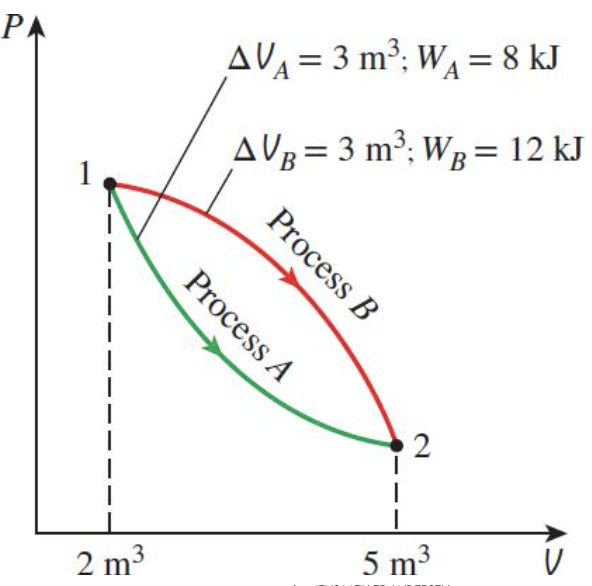
\includegraphics[width=0.35\linewidth]{./figures/f2_1.png}
  \label{fig:f2_1}
\end{figure}

\section{Arbejde}
Arbejde er et mål for energioverførslen fra et system til et andet. Typisk defineres arbejde som integralet af produktet af en kraft og den strækning denne kraft tager. Eksempelvis er arbejdet for en aksel med kraftmoment $T$, radius $r$ og omdrejningshastighed $\dot{n}_{\mathrm{omdr}}$ givet ved
\[ 
W_a = \mathrm{kraft} \cdot \mathrm{vej} = \frac{T}{r} \left( 2 \cdot \pi \cdot r \cdot n_{\mathrm{omdr}} \right) = 2\pi \cdot T \cdot n_{\mathrm{omdr}}
.\]
På samme vis kan arbejdet af en fjeder med der er strukket fra $x_{1}$ til $x_2$ og leverer en kraft på $F(x)$ overalt findes som
\[ 
W_f = \int \mathrm{kraft} \cdot \mathrm{vej} = \int_{x_1}^{x_2} F \, \mathrm{d}x = \frac{1}{2} k \left( x_2^2 - x_1^2 \right)
.\]

\subsection{Virkningsgrad}
Virkningsgraden $\eta$ for et system er defineret som forholdet mellem det opnåede output og det input der kommes ind i et system eller en maskine. Altså
\[ 
\eta = \frac{\text{Faktisk output}}{\mathrm{Input}}
.\]

